%! TEX root = 3_slab.tex
% the main TeX file which is intended to compile, :VimtexReload after adjustment
   % this file should be included in the main file
% :h vimtex-tex-root
\documentclass[../modul_skb.tex]{subfiles}
%ensure the class of docs

\begin{document}

\section{Plat Lantai}%
\label{sec:Plat Lantai}

Pelat Lantai adalah lantai yang tidak terletak diatas tanah langsung, merupakan lantai tingkat pembatas antara tingkat yang satu dengan tingkat yang lain. Pelat lantai didukung oleh balok-balok yang bertumpu pada kolom-kolom bangunan. Pelat lantai adalah struktur yang pertama kali menerima beban baik itu beban mati maupun beban hidup yang kemudian menyalurkannya ke sistem struktur rangka yang lain. Pekerjaan pelat lantai ini haruskah kokoh, kaku, mempunyai ketinggian yang sama dan nyaman untuk berpijak (A.L. Fatin, 2014a). Ketebalan pelat lantai ini disesuaikan dengan beberapa hal, diantaranya :

\begin{itemize}
	\item Beban yang akan ditumpu
	\item Lebar bentangan atau jarak antara balok-balok penumpu
	\item Bahan material konstruksi pelat lantai
	\item Besar lendutan yang diinginkan
\end{itemize}

\subsection{Jenis-Jenis Pelat Lantai}%
\label{sub:Jenis-Jenis Pelat Lantai}

Berdasarkan material bahannya terdapat bermacam – macam dari pelat lantai. Macam – macam pelat lantai tersebut, yaitu :

\subsubsection{Pelat Lantai Kayu}%
\label{ssub:Pelat Lantai Kayu}

Pelat lantai kayu ini tebuat dari bahan kayu yang dirangkai dan disatukan menjadi satu kesatuan yang kuat, sehingga terbentuklah bidang injak yang luas.

\begin{figure}
	\begin{center}
		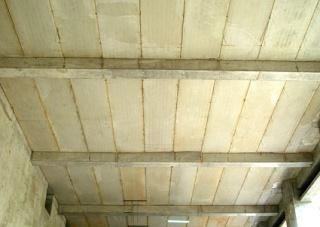
\includegraphics[width=.82\textwidth]{../figures/pelat_kayu.jpg}
		% filename may not contain space but _
	\end{center}
	\caption{Pelat Lantai Kayu}
	\label{fig:pelatkayu}
\end{figure}

Pelat lantai kayu ini terbuat dari bahan kayu, yang dirangkai dan disatukan menjadi satu kesatuan yang kuat, sehingga terbentuklah bidang injak yang luas. Pelat lantai kayu pada umumnya mempunyai ukuran-ukuran yang umum di pasaran. Ukuran-ukuran tersebut antara lain:

\begin{tabular}{l l}
	\hline
	Lebar papan kayu             &  : 20-30cm  \\
	Tebal papan kayu             &  : 2-3 cm  \\
	Jarak antar balok pendukung  &  : 60 – 80 cm  \\
	Ukuran balok                 &  : 8/12 , 8/14 dan 10/14  \\
	Bentangan                    &  : 3 – 3,5 cm  \\
	Berat jenis                  &  : 0,6 – 0,8 (t/m)  \\
\end{tabular}

Balok-balok kayu ini bisa diletakkan diatas pasangan 1 batu bata ataupun diatas balok beton. Pelat lantai kayu memiliki kelebihan dan kekurangannya sendiri. Berbagai kelebihan dan kekurangan pelat lantai kayu yaitu:

\begin{itemize}
	\item Kelebihan :
	      \begin{itemize}
		      \item Ekonomis, karena harganya yang relatif murah
		      \item Hemat ukuran pondasi, dikarenakan beratnya yang ringan Mudah dikerjakan.
	      \end{itemize}

	\item Kekurangan :
	      \begin{itemize}
		      \item Hanya diperbolehkan untuk struktur konstruksi bangunan yang sederhana dan ringan
		      \item Bukan benda peredam suara yang baik, karena itu suara langkah kaki yang ditimbulkan di lantai atas bisa terdengar oleh penghuni yang sedang berada di lantai bawahnya sehingga mengganggu penghuninya.
		      \item Mempunya sifat yang mudah terbakar
		      \item Tidak tahan air atau mudah bocor, sehingga tidak cocok untuk lantai kamar mandi / WC.
		      \item Tidak tahan lama / tidak awet, karena bisa dimakan oleh serangga pemakan kayu.
		      \item Mudah terpengaruh oleh cuaca, seperti hujan, panas, dll. Tidak dapat dipasangi keramik.
		      \item Tidak dapat dipasangi keramik (A.L Fatin, 2014b).
	      \end{itemize}

\end{itemize}

\subsubsection{Pelat Lantai Beton}%

Pelat lantai beton ini umumnya bertulang dan dicor ditempat bersama dengan balok penumpu dan kolom pendukungnya.

Yang dimaksud dengan pelat beton bertulang yaitu struktur tipis yang dibuat dari beton bertulang dengan bidang yang arahnya horizontal, dan beban yang bekerja tegak lurus pada bidang struktur tersebut. Ketebalan bidang pelat ini relatif sangat kecil apabila dibandingkan dengan bentang panjang/lebar bidangnya. Pelat beton bertulang ini sangat kaku dan arahnya horizontal, sehingga pada bangunan gedung, pelat ini berfungsi sebagai diafragma/unsur pengaku horizontal yang sangat bermanfaat untuk mendukung ketegaran balok portal.

\begin{figure}
	\begin{center}
		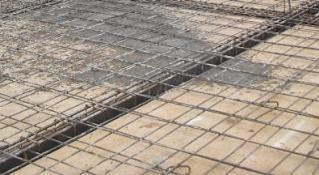
\includegraphics[width=.82\textwidth]{../figures/pelat_beton.jpg}
		% filename may not contain space but _
	\end{center}
	\caption{Pelat Lantai Beton}
	\label{fig:pelatbeton}
\end{figure}


Pelat lantai beton ini mempunyai beberapa keunggulan / keuntungannya sendiri, antara lain:

\begin{itemize}
	\item Mendukung untuk digunakan pada bangunan dengan beban yang besar
	\item Tidak dapat terbakar dan kedap air, sehingga dapat dijadikan sebagai lantai dapur, kamar mandi ataupun WC
	\item Dapat dipasang keramik, tegel dan granit, sehingga dapat memperindah lantai
	\item Bahan yang awet dan kuat, perawatannya mudah dan berumur panjang merupakan isolasi suara yang baik.
\end{itemize}

\subsection{Klasifikasi Pelat Lantai}


Pada umumnya struktur pelat beton dalam suatu bangunan gedung dapat diklasifikasikan menjadi tiga kelompok:

\subsubsection{Pelat Satu Arah}

Jika sistem pelat hanya ditumpu di kedua sisinya, makal pelat akan melentur atau mengalami lendutan dalam arah tegak lurus dari sisi tumpuan. Beban akan didistribusikan oleh pelat dalam satu arah saja yaitu ke arah tumpuan. Pelat jenis ini disebut juga pelat satu arah. Apabila pelat tertumpu di keempat sisinya, dan rasio bentang panjang terhadap bentang pendek lebih besar atau sama dengan 2, maka hampir 95\% beban akan dilimpahkan dalam arah bentang pendek, dan pelat akan menjadi sistem pelat satu arah. Sistem pelat satu arah cocok digunakan pada bentangan 3-6 meter, dengan beban hidup sebesar 2,5-5 kN/m2.

\subsubsection{Sistem Pelat Rusuk (Joist Construction)}

Sistem pelat rusuk terdiri dari pelat beton dengan ketebalan 50 hingga 100 mm yang ditopang oleh sejumlah rusuk dengan jarak beraturan. Rusuk mempunyai lebar minimum 100 mm dan mempunyai tinggi tidak lebih dari 3,5 kali lebar minimumnya. Rusuk biasanya bersisi miring dan disusun dalam jarak tertentu yang tidak melebihi 750 mm. Rusuk biasanya ditopang oleh balok induk utama yang langsung menumpu pada kolom. Sistem pelat rusuk cocok digunakan untuk struktur pelat dengan bentangan 6-9 m serta memikul beban hidup sebesar 3,5-5,5kN/m2 (Agus Setiawan, 2016a, p.252).

\subsubsection{Pelat Dua Arah}%

Apabila struktur pelat beton ditopang dikeempat sisinya, dan rasio antara bentang panjang terhadap bentang pendeknya kurang dari 2, maka pelat dikategorikan sebagai sistem pelat dua arah. Sistem pelat dua arah dapat dibedakan menjadi beberapa jenis sebagai berikut:


\begin{itemize}
	\item Sistem balok-pelat dua arah
	\item[] Pada sistem ini pelat beton ditumpu oleh balok dikeempat sisinya. Beban dari pelat ditransfer ke keempat balok penmpu yang selanjutnya mentransfer bebannya ke kolom. Sistem pelat dua arah dengan balok ini dapat digunakan untuk bentangan 6-9 meter, dengan beban hidup sebesar 2,5-5,5 kN/m2. Balok akan meningkatkan kekakuan pelat, sehingga lendutan yang terjadi akan relatif kecil.
	\item Sistem slab datar (flat slab)
	\item[] Sistem ini tidak memiliki balok penumpu di masing-masing sisinya. Beban pelat ditransfer langsung ke kolom. Kolom cenderung akan menimbulkan kegagalan geser pons pada pelat, yang dapat dicegah dengan beberapa alternatif:
\end{itemize}

\begin{itemize}
	\item Memberikan penebalan setempat pada pelat (drop panel) serta menyediakan kepala kolom (column capital)
	\item Menyediakan penebalan panel namun tanpa kepala kolom, panel disekitar kolom harus cukup tebal untuk memikul terjadinya tegangan tarik diagonal yang muncul akibat geser pons.
	\item Menggunakan kepala kolom tanpa ada penebalan panel.
\end{itemize}

Sistem slab datar dapat digunakan untuk bentangan 6-9 meter, dengan beban hidup sebesar 4-7 kN/m2. 3) Sistem pelat datar (flat plate).

Sistem ini terdiri dari pelat yang tertumpu langsung ke kolom tanpa adanya penebalan panel dan kepala kolom. Potensi kegagalan struktur terbesar akan timbul akibat geser pons, yang akan menghasilkan tegangan tarik diagonal. Sebagai akibat tidak adanya penebalan panel dan kepala kolom, maka dibutuhkan ketebalan pelat yang lebih besar atau dengan memberikan penulangan ekstra diarea sekitar kolom. Sistem slab datar dapat digunakan untuk struktur pelat dengan bentangan 6-7,5 meter, dengan beban hidup sebesar 2,5-4,5 kN/m2.

\begin{itemize}
	\item Pelat dua arah berusuk dan pelat waffle
	\item[] Ini merupakan sistem pelat dua arah dengan ketebalan pelat antara 50 mm hingga 100 mm yang ditumpu oleh rusuk-rusuk dalam dua arah. Jarak antar rusuk berkisar antara 500 mm hingga 750 mm. Tepi-tepi pelat dapat ditopang oleh balok, atau dapat juga pelat langsung menumpu pada kolom dengan memberikan penebalan pada pelat disekitar kolom \end{itemize}

\subsection{Tumpuan Pelat}%
\label{sub:Tumpuan Pelat}
Untuk merencanakan pelat beton bertulang perlu dipertimbangkan jenis perletkan dan jenis penghubung di tempat tumpuan. Kekakuan hubungan antara pelat dan tumpuan akan menentukan besar momen lentur yang terjadi pada pelat.

Untuk bangunan gedung, umumnya pelat ditumpu oleh balok-baloik dengan berbagai sistem sebagai berikut:

\begin{itemize}
	\item Monolit, yaitu pelat dan balok dicor bersama-sama sehingga menjadi satu kesatuan. Gambar~\ref{fig:tumpuan_balok}
	\item Ditumpu dinding-dinding / tembok bangunan. Gambar~\ref{fig:tumpuan_balok}
	\item Didukung oleh balok-balok baja dengan sistem komposit. Gambar~\ref{fig:tumpuan_baja}
	\item Didukung oleh kolom secara langsung tanpa balok, dikenal dengan pelat cendawan. Gambar~\ref{fig:tumpuan_baja}
\end{itemize}


\begin{figure}
	\begin{center}
		
\includegraphics[width=.82\textwidth]{tumpuan_balok}
		% filename may not contain space but _
	\end{center}
	\caption{Pelat Ditumpu Balok (Monolit) dan Pelat Ditumpu Dinding Tembok}
	\label{fig:tumpuan_balok}
\end{figure}

\begin{figure}
	\begin{center}
		
\includegraphics[width=.82\textwidth]{tumpuan_baja}
		% filename may not contain space but _
	\end{center}
	\caption{Pelat Ditumpu Balok Baja dengan Sistem Komposit dan Secara Langsung}
	\label{fig:tumpuan_baja}
\end{figure}


\subsection{Metode Pelaksanaan Pelat Lantai}%

\subsubsection{Metode Konvensional}

Metode konvensional yaitu pengerjaan pembetonan dilakukan secara manual di tempat (\textit{cast in place}). Langkah-langkah pengerjaan pengecoran pelat lantai dengan metode konvensional yaitu:

\begin{itemize}
	\item Pemasangan perancah / \textit{scaffolding}
	\item Pemasangan bekisting
	\item Perakitan tulangan / pembesian
	\item Pengecoran
\end{itemize}

Kelebihan beton konvensional:

\begin{itemize}
	\item Lebih mudah disesuaikan dengan kebutuhan
	\item Dapat dibuat di tempat yang sempit
	\item Pengawasan lebih mudah dan terkontrol
\end{itemize}

Kekurangan beton konvensional:

\begin{itemize}
	\item Waktu pengerjaan lebih lama
	\item Membutuhkan banyak tenaga kerja
	\item Kualitas dan mutu sulit terukur
	\item Kurang ramah lingkungan karena terdapat limbah dari sisa-sisa pengerjaan seperti bekisting kayu
	\item Pengaruh cuaca relatif besar
\end{itemize}



\subsubsection{Metode Full Precast}

Metode full precast adalah metode pengerjaan pelat lantai dengan seluruh komponen pelat menggunakan beton pracetak. Beton pracetak merupakan teknologi konstruksi struktur beton dengan komponen-komponen penyusun yang dicetak terlebih dahulu pada suatu tempat khusus (\textit{off-site fabrication}). Dalam beberapa kasus, komponen-komponen tersebut dapat dirakit terlebih dahulu (\textit{pre-assembly}), kemudian dipasang di lokasi proyek (\textit{installation}).

Dengan demikian, sistem pracetak berbeda dengan konstruksi monolit terutama pada aspek perencanaan yang juga dipengaruhi oleh metode pelaksanaan pabrikasi, proses penyatuan dan pemasangan, serta perilaku teknis sistem pracetak dalam hal sambungan antar komponen (\textit{joint}) (Abduh, 2007, dikutip dalam Perkembangan Beton Pracetak, 2014).

Menurut Hendrawan Wahyudi dan Hery Dwi Hanggoro (2010), struktur elemen pracetak memiliki beberapa keuntungan dibandingkan dengan struktur konvensional.

Kelebihan beton precast:

\begin{itemize}
	\item Penyederhanaan pelaksanaan konstruksi
	\item Waktu pelaksanaan lebih cepat
	\item Penggunaan material lebih optimum serta mutu bahan lebih baik
	\item Penggunaan cetakan dapat dilakukan berulang-ulang
	\item Penyelesaian \textit{finishing} lebih mudah
	\item Tidak membutuhkan lahan proyek yang luas, mengurangi kebisingan, lebih bersih, dan lebih ramah lingkungan
\end{itemize}

Kelemahan beton precast:

\begin{itemize}
	\item Tidak ekonomis untuk produksi dalam jumlah kecil
	\item Panjang dan bentuk elemen pracetak terbatas sesuai kapasitas alat angkat dan alat angkut
	\item Memerlukan ruang yang cukup bagi pekerja untuk mengerjakan sambungan beton pracetak
	\item Memerlukan lahan yang cukup luas untuk proses pabrikasi dan penimbunan
	\item Hanya dapat dilaksanakan di daerah yang telah tersedia peralatan untuk \textit{handling} dan \textit{erection}
	\item Jarak maksimum transportasi yang ekonomis menggunakan truk sekitar 150–350 km, tergantung tipe produknya
	\item Untuk transportasi laut, jarak maksimum dapat mencapai lebih dari 1000 km
	\item Pada daerah rawan gempa, konstruksi beton pracetak memiliki risiko pada bagian sambungan sehingga perencanaan sambungan menjadi aspek yang sangat penting
\end{itemize}

Metode ini merupakan salah satu metode dengan waktu pelaksanaan paling cepat. Namun demikian, beberapa hal perlu diperhatikan, antara lain kualitas sambungan beton pracetak, proses transportasi elemen pracetak ke lokasi proyek, serta kapasitas alat angkat. Kapasitas angkat ujung \textit{tower crane} harus lebih besar dari total berat elemen beton pracetak yang diangkat.


\subsubsection{Metode Half Slab}

Metode ini disebut metode \textit{half slab} karena sebagian struktur pelat lantai dikerjakan dengan sistem precast. Bagian tersebut dibuat di pabrik kemudian dikirim ke lokasi proyek untuk dipasang sebagai lapisan pertama yang sekaligus berfungsi sebagai bekisting. Setelah itu dilanjutkan dengan perakitan tulangan dan pengecoran lapisan kedua pelat lantai yang dilakukan langsung di lapangan.

Kelebihan pelat lantai metode \textit{half slab}:

\begin{itemize}
	\item Waktu pengerjaan lebih cepat dibandingkan pelat lantai sistem konvensional
	\item Efisiensi penggunaan material bekisting karena beton pracetak berfungsi sebagai bekisting
	\item Tidak menggunakan kayu sehingga lebih mendukung konsep \textit{green building} dan lebih ramah lingkungan
\end{itemize}

Kekurangan pelat lantai metode \textit{half slab}:

\begin{itemize}
	\item Sulit diaplikasikan pada area tepi gedung (kantilever)
	\item Memerlukan teknik khusus jika digunakan pada area toilet atau atap gedung agar tidak terjadi kebocoran
	\item Memerlukan proses pengiriman beton pracetak dari pabrik ke lokasi proyek
	\item Keterbatasan kapasitas alat angkat untuk mengangkat elemen beton pracetak (Ahadi, 2013)
\end{itemize}

\subsubsection{Metode Bondek}

Metode bondek merupakan metode pelaksanaan pelat lantai dengan mengganti tulangan bagian bawah menggunakan pelat bondek yang sekaligus berfungsi sebagai bekisting. Setelah pemasangan bondek, pekerjaan dilanjutkan dengan perakitan tulangan bagian atas dan pengecoran struktur bagian atas pelat lantai. Penggantian tulangan bawah dengan pelat bondek diharapkan dapat menghemat penggunaan besi tulangan dan material bekisting.

Kelebihan pelat lantai metode bondek:

\begin{itemize}
	\item Efisiensi penggunaan material bekisting karena pelat bondek berfungsi sebagai bekisting
	\item Tidak menggunakan besi tulangan bagian bawah karena fungsinya telah digantikan oleh bondek
	\item Waktu pengerjaan lebih cepat dibandingkan sistem konvensional
	\item Bagian bawah pelat lantai lebih rapi
	\item Pelat bondek relatif aman terhadap kebakaran
	\item Pelat bondek memiliki sifat anti karat
	\item Tidak membutuhkan banyak tenaga kerja pada proses pemasangan
\end{itemize}

Kekurangan pelat lantai metode bondek:

\begin{itemize}
	\item Tidak dapat diterapkan pada sisi tepi gedung (pelat lantai kantilever)
	\item Membutuhkan keahlian khusus dalam pemasangan untuk menghindari kemungkinan material bondek terbuang
	\item Harga dipengaruhi oleh perkembangan harga baja
	\item Pemasangan sambungan antar sisi bondek harus menggunakan las listrik untuk memperkuat sambungan.
\end{itemize}















\bibliographystyle{apalike}
\bibliography{../filename.bib} % required for citecompletion, not work in mainfile
\end{document}

